% !Mode:: "TeX:UTF-8"

\chapter{红外无人机目标检测算法}

\section{引言}
本课题研究的红外无人机目标检测问题,主要需要解决的问题有两个。
一个是原始图像是由红外设备产生的,因此原始图片是灰度图,
不含有普通BGR图像的三个通道信息;
另一个问题是在实际的检测场景下,无人机目标在检测设备中往往以小目标形式出现,
本课题对算法小目标的检测能力要求较高。
因此本章所做的研究首先是针对本课题的红外无人机目标检测问题
建立研究必要的数据集,
之后选择一种在该数据集上性能较好的深度学习算法
作为基础算法,接着针对上述的两个问题提出了
基于通道填充和图像合成的数据增强算法,
在mAP和推理时间两个方面
进一步提升算法在数据集上的性能表现。

\section{数据集制作}[Number]
由于神经网络需要大量的数据进行训练,
并且算法还需要在数据集上进行测试,
因此本课题研究需要一个红外无人机目标的数据集。
由于目前尚无开源红外无人机数据集可供使用,
本课题自建了红外无人机数据集。

\subsection{数据集概况}
目前国内外完善标注的公开红外数据集很少,
仅有少量红外无人机数据集但多以点标注形式发布,
因此需要自行收集红外无人机图像并进行标注。
考虑到网络模型的泛化能力和特征提取的鲁棒性,
自行收集了多种背景的红外图像,
并且覆盖距离远近的无人机目标,目标全部为旋翼无人机。
数据集来源主要是网络获取和实验室自主采集两种方式,
格式为红外无人机图像和视频,通过脚本转换为图片格式后,
标注目标框,制作成数据集,总共包含10000张图片,原始格式为PASCAL VOC,
按训练集、验证集、测试集划分分别有7000张、2000张、1000张。
数据集中的原图示例如图\ref{dataset}所示。

\begin{figure}[!h]
    \setlength{\subfigcapskip}{-1bp}

    \centering
    \begin{minipage}{\textwidth}
    \centering
    \subfigure{\label{dataset11}}\addtocounter{subfigure}{-2}
    \subfigure{\subfigure[正常目标示例~1]{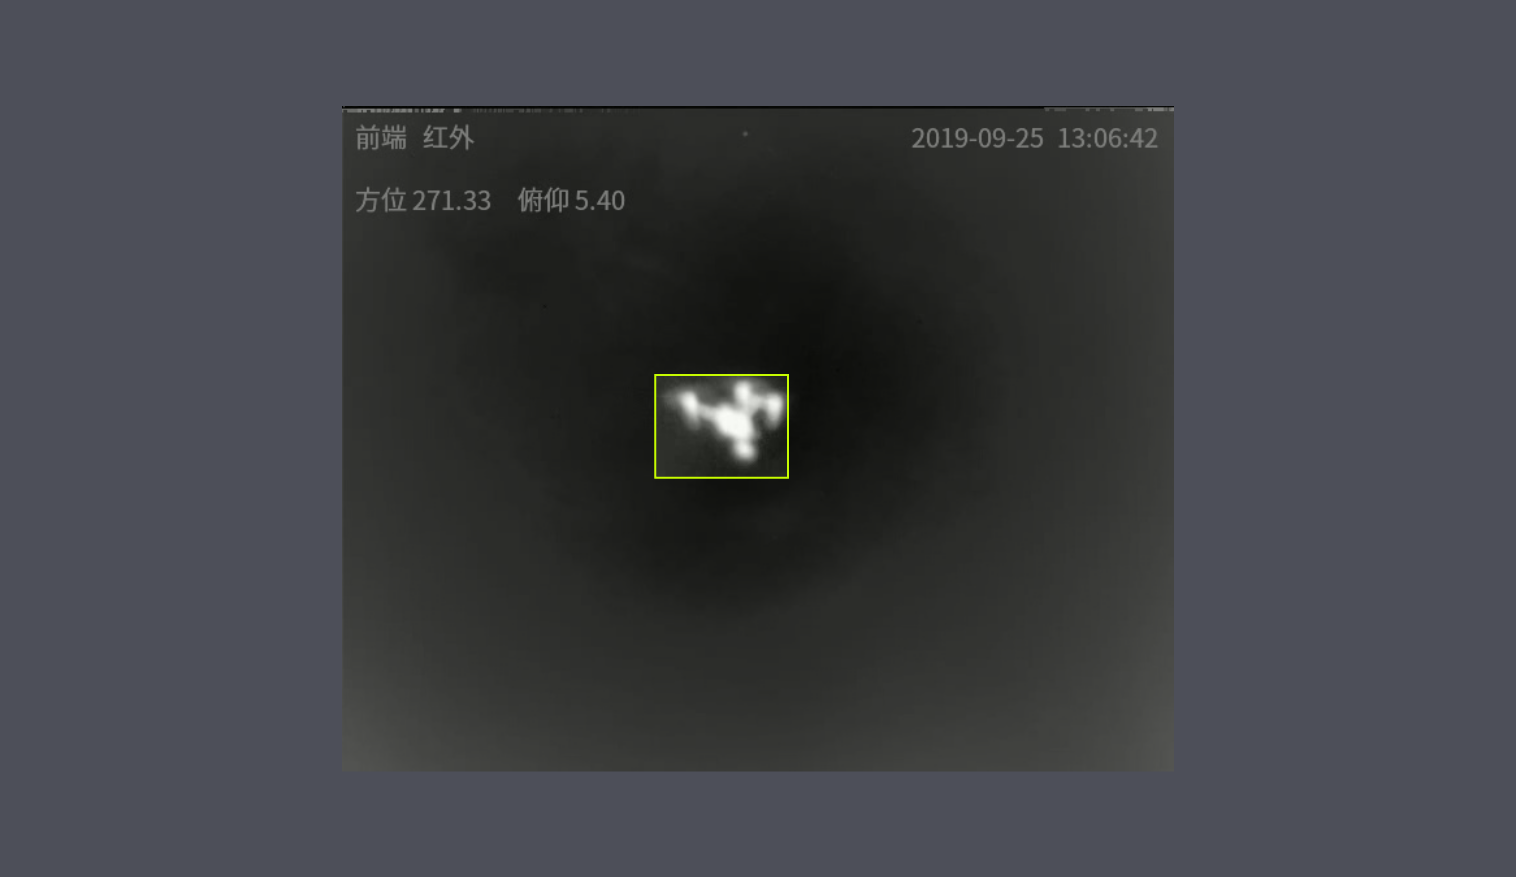
\includegraphics[width=0.4\textwidth]{1.png}}}
    \hspace{2em}
    \subfigure{\label{dataset12}}\addtocounter{subfigure}{-2}
    \subfigure{\subfigure[正常目标示例~2]{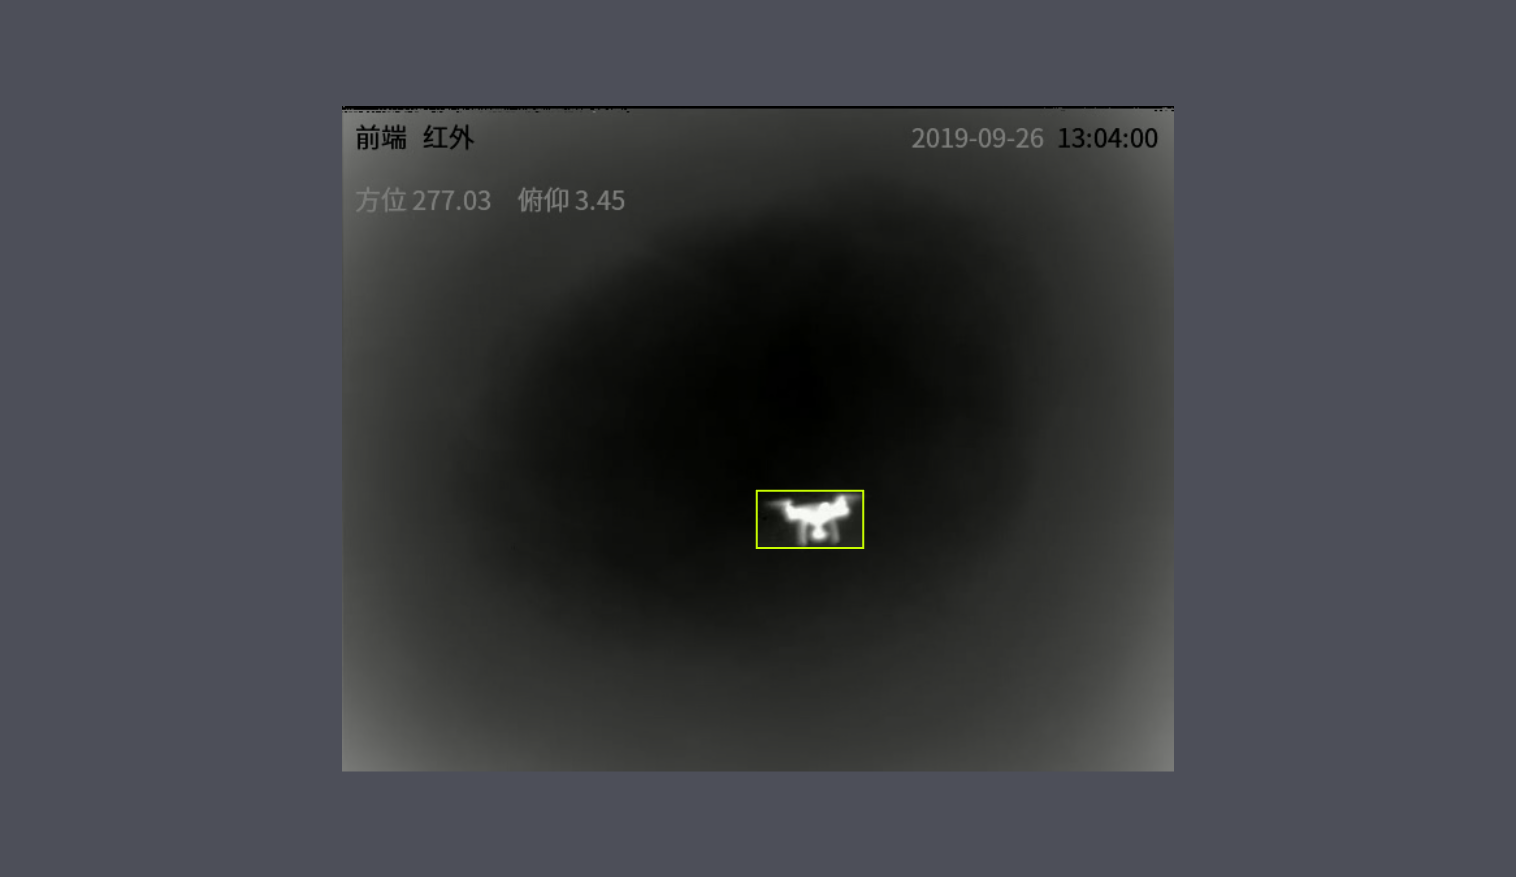
\includegraphics[width=0.4\textwidth]{2.png}}}
    \end{minipage}

    \centering
    \begin{minipage}{\textwidth}
    \centering
    \subfigure{\label{dataset21}}\addtocounter{subfigure}{-2}
    \subfigure{\subfigure[小目标示例~1]{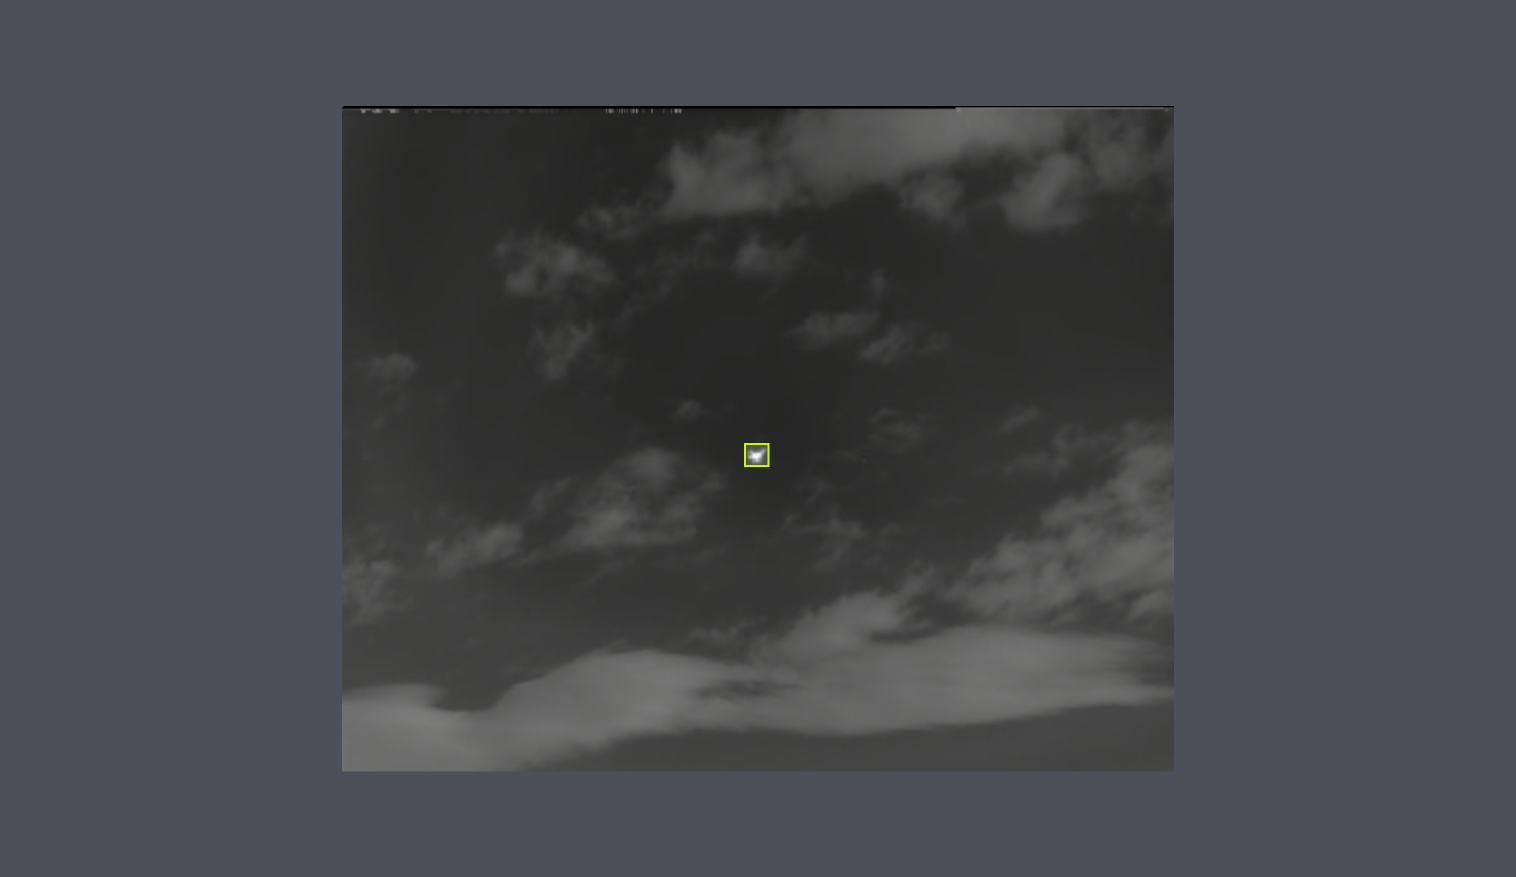
\includegraphics[width=0.4\textwidth]{5.png}}}
    \hspace{2em}
    \subfigure{\label{dataset22}}\addtocounter{subfigure}{-2}
    \subfigure{\subfigure[小目标示例~2]{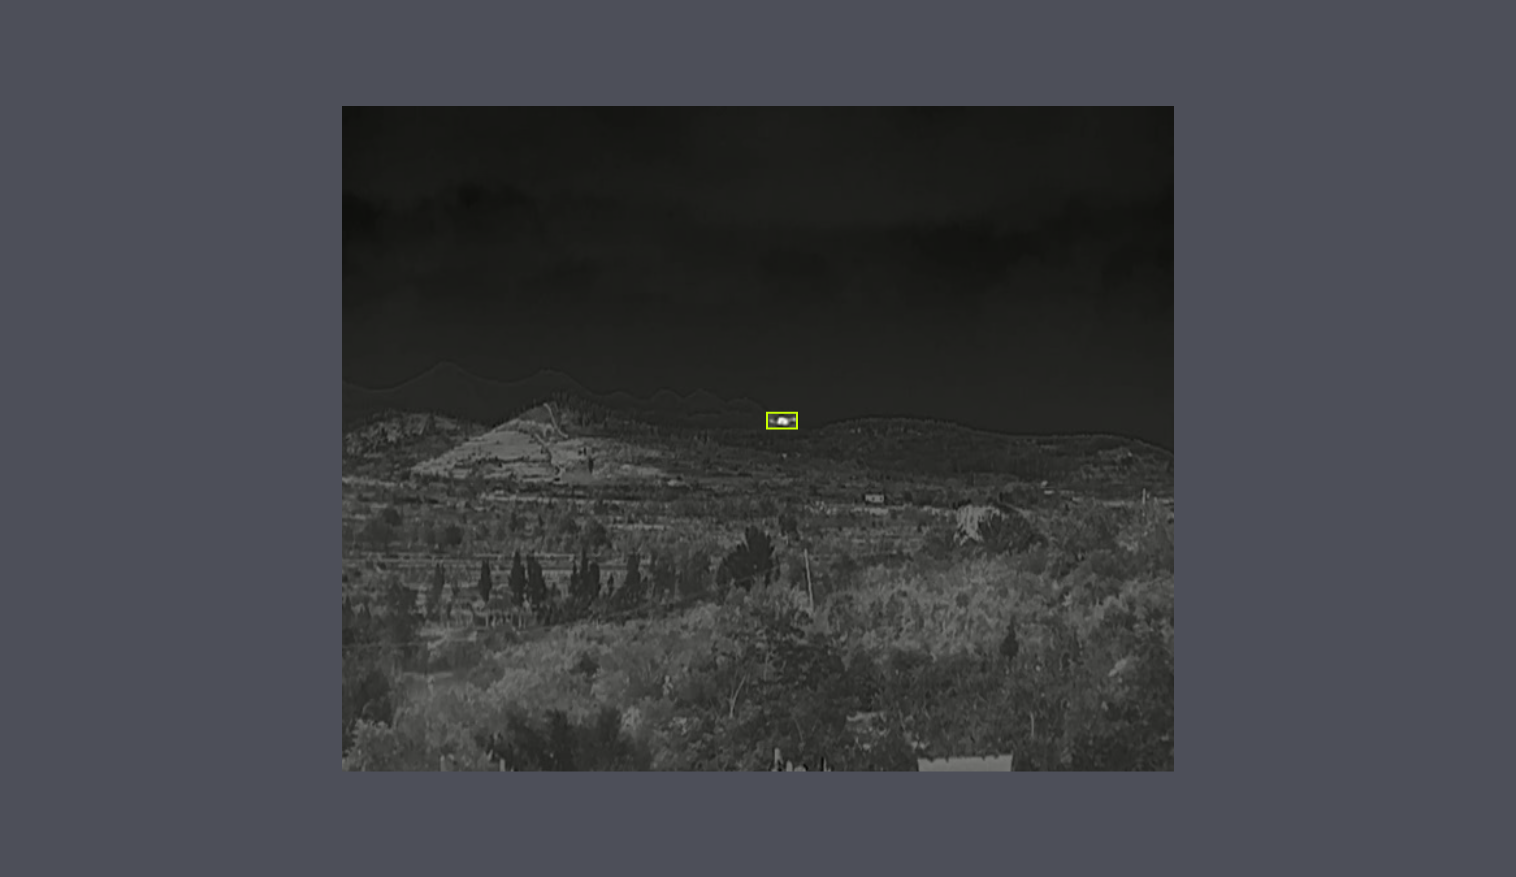
\includegraphics[width=0.4\textwidth]{6.png}}}
    \end{minipage}

    \centering
    \begin{minipage}{\textwidth}
    \centering
    \subfigure{\label{dataset31}}\addtocounter{subfigure}{-2}
    \subfigure{\subfigure[遮挡目标示例~1]{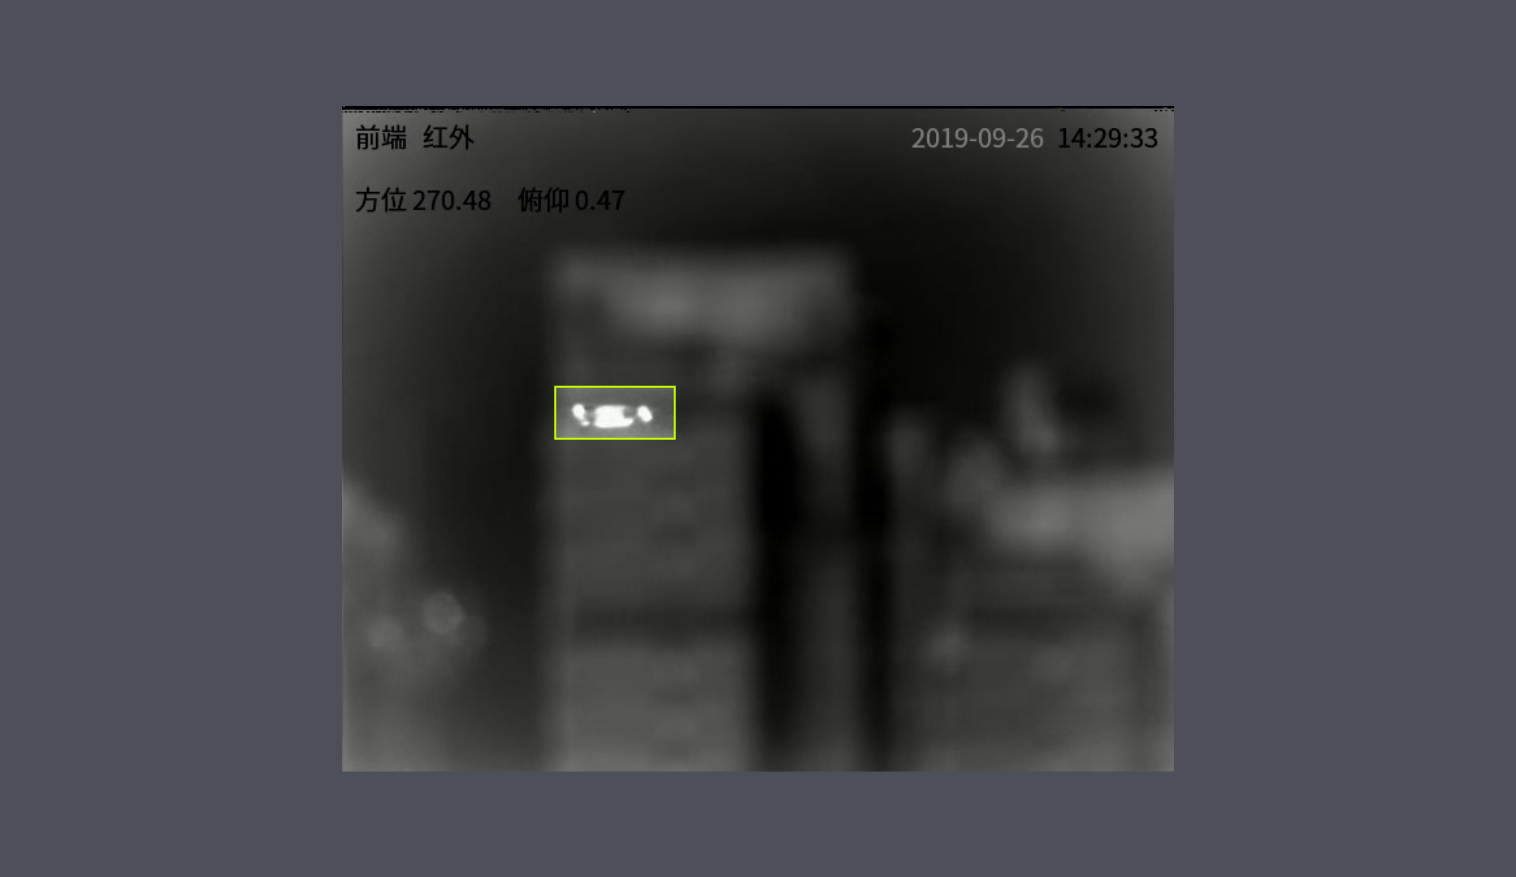
\includegraphics[width=0.4\textwidth]{3.png}}}
    \hspace{2em}
    \subfigure{\label{dataset32}}\addtocounter{subfigure}{-2}
    \subfigure{\subfigure[遮挡目标示例~2]{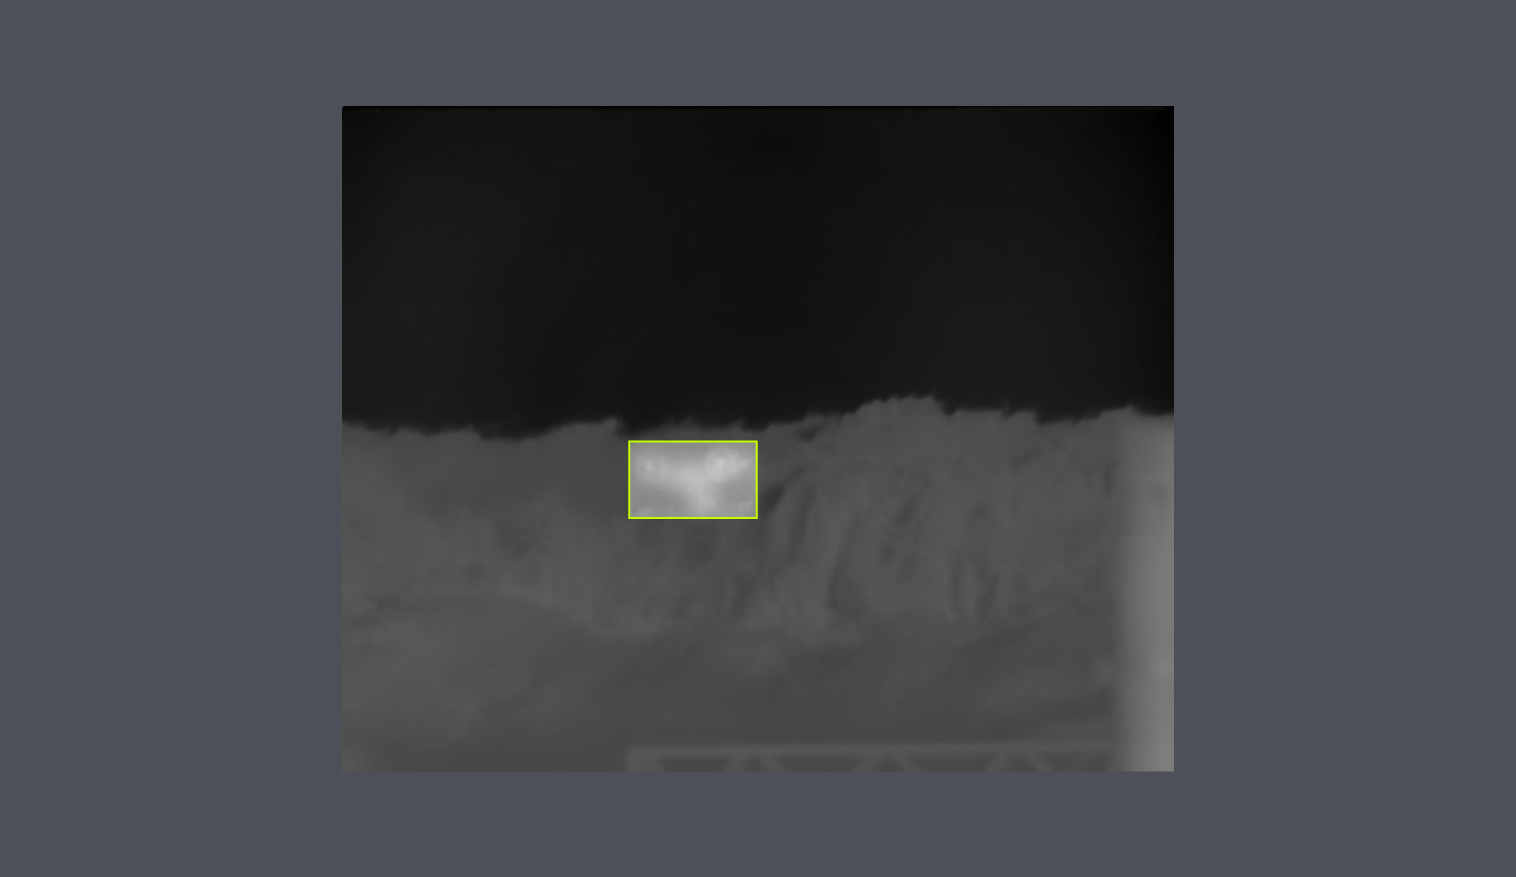
\includegraphics[width=0.4\textwidth]{4.png}}}
    \end{minipage}

    \vspace{0.2em}
    \caption{数据集图像示例}
    {\label{dataset}}
\end{figure}


\section{深度学习网络模型基本算法YOLOv5}
本课题算法的主干网络模型采用YOLOv5网络,网络的结构如图\ref{yolo1}所示,
该模型按照推理流程顺序主要可以分成
输入端、Backbone、Neck、Prediction这四个部分。

\begin{figure}[h]
    \centering
    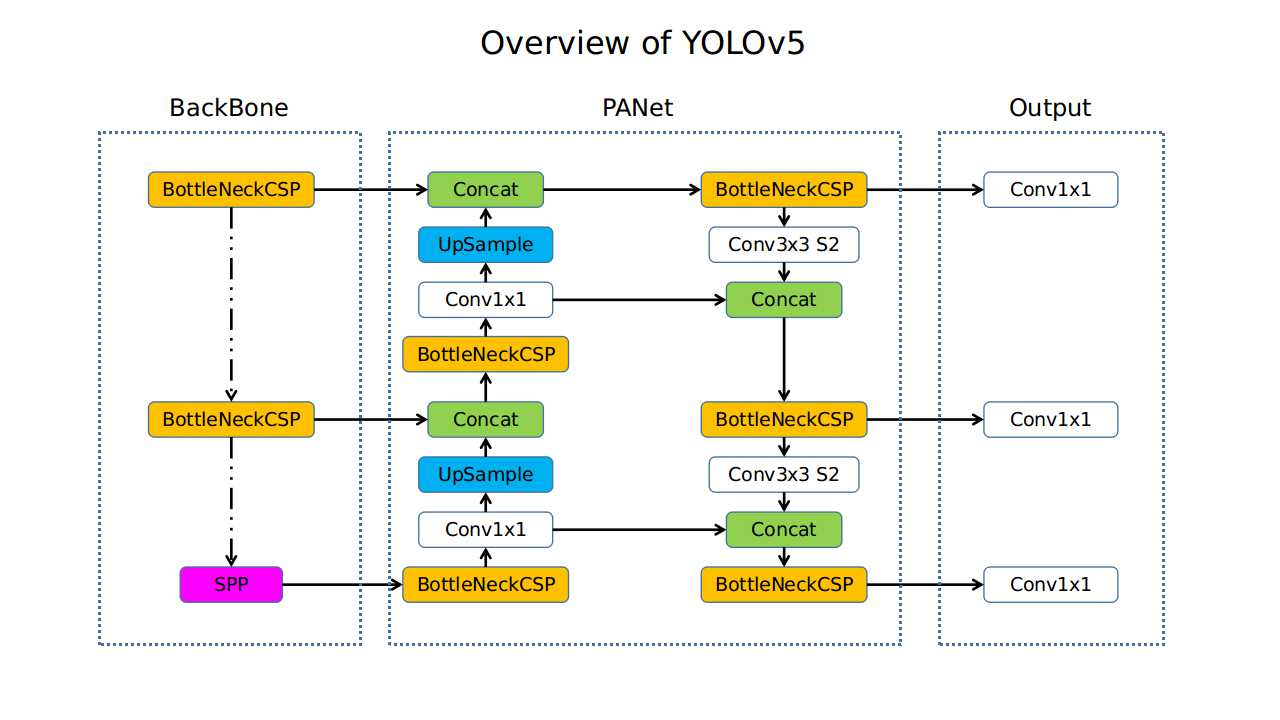
\includegraphics[width = 0.8\textwidth]{yolov5结构.jpg}
    \caption{yolov5网络结构}
    \label{yolo1}
\end{figure}

\subsection{输入端}
YOLOv5网络的输入端就是输入图像的模块,
既可以向网络提供原始的图像输入,
也可以在这个部分对图像进行预处理
和数据增强,
此外还能进行算法的准备工作,比如锚框的
自适应计算等。

\subsection{Backbone}
Backbone的主要作用是初步提取特征图。其中典型的模块是Focus模块、CBL模块以及CSP模块。

\subsubsection{Focus模块}
Focus模块在YOLOv5中是图片进入backbone前,对图片进行切片操作,
具体操作是在一张图片中每隔一个像素拿到一个值,类似于邻近下采样,
这样就拿到了四张图片,四张图片互补,长的差不多,但是没有信息丢失,
这样一来,将W、H信息就集中到了通道空间,输入通道扩充了4倍,
即拼接起来的图片相对于原先的RGB三通道模式变成了12个通道,
最后将得到的新图片再经过卷积操作,最终得到了没有信息丢失情况下的二倍下采样特征图。

\begin{figure}[h]
  \centering
  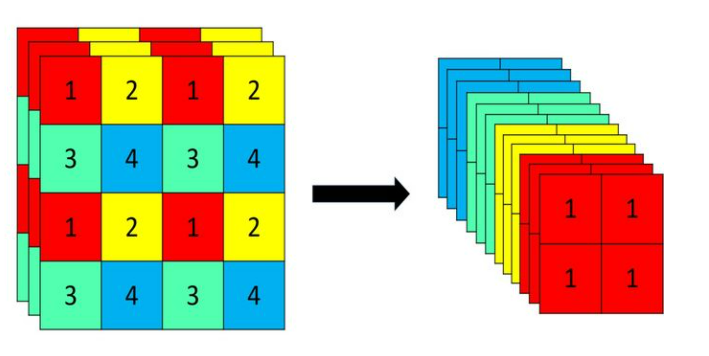
\includegraphics[width = 0.8\textwidth]{focus.png}
  \caption{Focus切片示意图}
  \label{focus}
\end{figure}

\subsubsection{CBL模块}
CBL模块是卷积神经网络的基本组成模式,
结构如图\ref{cbl}所示,
由卷积、归一化、激活函数三个部分组成。
CBL的主要作用是通过卷积采集特征。
其中的激活函数默认是Leaky ReLU,Leaky Rectified Linear Unit是一种基于 ReLU 的激活函数,但它对于负值的斜率很小,而不是平缓的斜率。 斜率系数是在训练之前确定的,即它不是在训练期间学习的。 这种类型的激活函数在我们可能遭受稀疏梯度的任务中很受欢迎。

\begin{figure}[h]
  \centering
  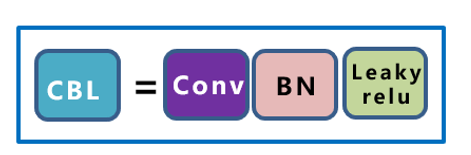
\includegraphics[width = 0.5\textwidth]{CBL.png}
  \caption{CBL模块组成示意图}
  \label{cbl}
\end{figure}

\begin{figure}[h]
  \centering
  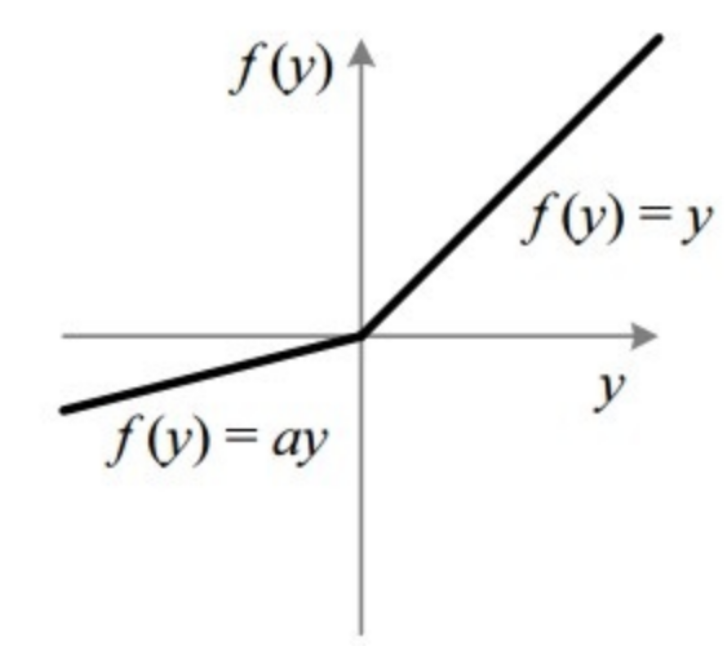
\includegraphics[width = 0.4\textwidth]{leakyrelu.png}
  \caption{Leaky ReLU示意图}
  \label{relu}
\end{figure}

\subsubsection{CSP模块}
SP结构从网络结构设计的角度来解决以往工作在推理过程中需要很大计算量的问题,CSP结构认为推理计算过高的问题是由于网络优化中的梯度信息重复导致的。CSP结构通过将基础层的特征图划分为两个部分,然后通过CSP结构将它们合并,可以在能够实现更丰富的梯度组合的同时减少计算量。
Yolov5使用CSPDarknet作为Backbone,从输入图像中提取丰富的信息特征。CSPNet解决了其他大型卷积神经网络框架Backbone中网络优化的梯度信息重复问题,将梯度的变化从头到尾地集成到特征图中,因此减少了模型的参数量和FLOPS数值,既保证了推理速度和准确率,又减小了模型尺寸。

\begin{figure}[h]
  \centering
  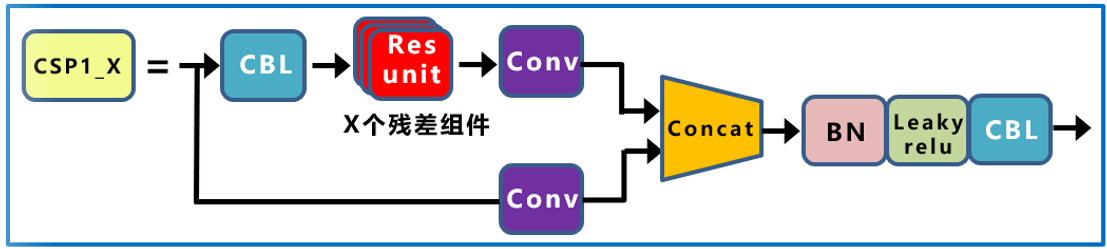
\includegraphics[width = 0.8\textwidth]{CSP.png}
  \caption{CSP模块组成示意图}
  \label{csp}
\end{figure}

\subsection{Neck}
Neck部分主要由FPN和PAN组成。FPN即特征金字塔网络(Feature Pyramid Network),特征金字塔是一种
用于检测不同尺度物体的系统。该算法模块利用固有的多尺度,
深度卷积网络的金字塔层次结构以边际额外成本构建特征金字塔。开发了具有横向连接的自上而下的架构,用于
在所有尺度上构建高级语义特征图。这种架构作为通用特征提取器在不同场景均显示出出色的性能。
FPN对小尺度目标检测效果更好。FPN可以利用经过top-down模型后的那些上下文信息(高层语义信息)。
对于小目标而言,FPN增加了特征映射的分辨率(即在更大的feature map上面进行操作,这样可以获得更多关于小目标的有用信息)。

PANet是一种旨在提升信息的路径聚合网络结构(Path Aggregation Network)。
具体来说,PANet增强了整个特征层次结构中
自下而上的低层精确定位信号,提出了自适应特征池,
它将特征网格和所有特征级别联系起来,进而在每个特征级别中生成有用的信息
直接传播到以下提议子网,缩短了较低层和最顶层特征之间的信息路径。
PANet在实例分割和目标检测等任务中均有着优秀的性能表现。

\subsection{Prediction}
Prediction部分包含上级输出的特征向量,并通过输入的特征向量得出坐标值、置信度,结合损失函数和后处理函数得出检测结果。

\section{YOLOv5基础网络性能验证与分析}
本节将在自建数据集上对YOLOv5基础网络的性能进行验证,将其与常见算法SSD和Faster RCNN进行对比,并分析YOLOv5算法的优势。

\subsection{实验环境与参数}
本章提到的YOLOv5基础算法用深度学习网络框架Pytorch进行实现、训练和测试。操作系统为Windows 10,使用的主要软件为python。实验平台采用的CPU型号为Intel Core i7-11700k,GPU型号为NVIDIA GeForce RTX 3080Ti,显存容量为12GB。训练过程中使用GPU进行加速。

\subsection{不同网络结构对比分析}
为了证明基础YOLOv5算法在红外无人机目标检测任务中的有效性,本节将其与目标检测算法SSD以及Faster RCNN进行对比实验。

\begin{table}[htbp]
  \caption{不同算法对红外无人机数据集的检测结果}
  \vspace{0.5em}\centering\wuhao
  \begin{tabular}{ccc}
  \toprule
  检测算法 & mAP & 推理时间\\
  \midrule
  YOLOv3 & 269.8 & 0.000674\\
  Faster-RCNN & 421.0 & 0.001035\\
  SSD & 640.2 & 0.001565\\
  YOLOv5 & 640.2 & 0.001565\\
  \bottomrule
  \end{tabular}
  \label{t1}
\end{table}

根据表\ref{t1}中的实验结果,Faster-RCNN相对于YOLOv3的检测精度更高,但是同时会消耗更多的推理时间。这是因为Faster-RCNN算法虽然相对于RCNN算法有所改进,但是仍然采用二阶段检测方式,先进行提名候选框后进行目标检测,这种检测方式虽然保证了检测精度,但是会使得算法总体的检测耗时较长。而YOLOv3的检测速度较快,这是由于YOLO系列算法直接采用了单阶段检测,较大程度地减少了推理时间,但是由于网络结构中没有充分利用多尺度特征信息,因此在尺度变化较大的数据集上精度不高。而SSD算法在单阶段检测的同时,引入了特征金字塔结构,充分利用了多尺度目标的特征,因而能在检测精度和推理时间上都有较好的表现。而YOLOv5网络在YOLOv3的基础上,应用了很多提升精度的改进,如增加了PANet、改进了损失函数等,也应用了很多提升速度的改进,如应用了CSP模块等,因此在实验结果中体现出YOLOv5的检测精度和推理时间都是最优的,因此本文选择YOLOv5算法作为红外无人机目标检测算法的基础。

\section{数据增强算法}
由于深度学习算法通常需要大量的数据进行学习,因此在原始数据集的基础上,将基础网络结合数据增强算法能在一定程度上提升算法的性能。因此本节将对常见的图像增强算法进行实验,在实验结果的基础上针对红外图像目标检测任务提出一种图像填充算法,此外还将针对红外无人机目标检测任务中的小目标占比较高的特性提出一种图像拼接的数据增强算法。

\subsection{主流的图像增强算法}
图像增强算法根据滤波方法不同分为空域增强算法和频域增强算法。空域增强算法是对图像的像素直接进行操作,常用的有直方图均衡、中值滤波器、拉普拉斯变化等,频域增强算法是以修改图像傅里叶变换为基础的,常用的有高通滤波器、低通滤波器等。由于空域增强算法相对简单,处理速度快,因此本课题采用的图像预处理算法都为空域增强算法,重点研究了几种具有代表性的空域增强算法。

由于空间域增强算法是采用不同的操作直接对像素进行处理,因此可以定义为:
\begin{equation}
  g(x, y)=T[f(x, y)]
\end{equation}

其中$f(x, y)$代表原始图像,$T$是作用在原图$(x, y)$邻域上的一种变换,$g(x, y)$表示处理过的图像。

\subsubsection{Inversion}
由于主流的目标检测算法应用的场景都是基于RGB图像的,不适于检测红外目标,因此需要将红外图像进行预处理以达到使红外图像更接近RGB图像的目的,通过域迁移的思想使得网络能够更加适应处理后的红外图像。一般用于目标检测所用的RGB图像都是白天所摄,通常情况是背景较亮,目标较暗。但是红外图像成像为辐射特性,故一般背景辐射较弱而目标辐射较强。因此,采用inversion操作:
\begin{equation}
  f: x_{p}=1-x
\end{equation}

\subsubsection{直方图均衡}
一般来说由于红外图像的对比度比较低因此导致其灰度分布通常都是分布在较窄的区域,与RGB图像的灰度分布不同,采用直方图均衡能够使红外图像的灰度分布更均匀从而达到增加图像细节信息的作用。针对直方图进行处理是多数空域处理技术中的重要手段,直方图均衡是对图像的灰度直方图进行非线性的拉伸,重新分配红外图像中的灰度值,从而增大红外图像的对比度,直方图均衡的步骤如下: 

(1)计算像素区间在$[0,L-1]$的图像灰度为:
\begin{equation}
  \mathrm{p}_{r}\left(r_{k}\right)=\frac{n_{k}}{n} \quad k=0,1,2, \ldots, L-1
\end{equation}

其中$n$代表图像的像素总数,$n_{k}$代表灰度级为$r_{k}$的像素个数。

(2)计算像素变换后的分布:
\begin{equation}
  \mathrm{s}_{k}=T\left(r_{k}\right)=\sum_{j=0}^{k} p_{r}\left(r_{j}\right)=\sum_{j=0}^{k} \frac{n_{j}}{n} \quad k=0,1,2, \ldots L-1
  \label{pix trans}
\end{equation}

通过式\ref{pix trans}可将图像中值为$r_{k}$的像素点映射到输出图像中值为$s_{k}$的点,此时$s_{k}$的像素值在$[0,1]$之间。

(2)将$s_{k}$转化为与原始图像灰度级一致:
\begin{equation}
  s_{k}=s_{k} *(L-1)
\end{equation}

直方图均衡对于太暗或太亮的图片都有很好的提高对比度效果,并且计算量不大,但该方法存在的局限在于变换后的图像灰度级会减少,造成细节信息的损失,严重的可能造成原本图像中的小目标丢失,后来针对以上问题发展出自适应直方图均衡(AHE),对比度受限的直方图均衡(CLAHE)等。

\subsubsection{USM锐化}
对于大多数情况下的目标检测任务,目标相对背景都是有较明显的轮廓,因此可以采用锐化处理方法进一步加强物体的边界,进而增强检测效果。

锐化的本质是对原图像实现高通滤波,得到原图像的高频分量,也就是对原图像中的边缘部分进行了增强。图像处理实现锐化有一种常用的算法USM(Unsharp Mask),这种锐化的方法就是对原图像先做一个高斯模糊取得原图像的低通分量,然后用原来的图像减去一个系数乘以高斯模糊之后的图像,然后再把值映射到$[0,255]$的RGB像素值范围之内。基于USM锐化的方法可以去除一些细小的干扰细节和噪声,比一般直接使用卷积锐化算子得到的图像锐化结果更加可靠。
\begin{equation}
  I_{sharpend}=I_{original}+(I_{original}-I_{blurred})*a
\end{equation}

式中$I_{sharpend}$表示锐化后的图像,$I_{original}$表示原始图像,$I_{blurred}$表示模糊后的原始图像,$a$表示权重系数。

\subsection{通道填充算法}
如前文所述,红外图像由于信噪比低等特点因此相对可见光图像来说信息量
少。本章针对红外图像的特点,结合前文介绍的图像增强手段,提出了一种基于
通道填充的红外图像数据增强算法,该算法的主要思想为:由于红外图像为单通
道图像,携带的信息量有限,选择另外两种红外图像增强方法将单通道的红外图像填充成
三通道,再输入到网络中,增加数据量的同时使网络能够学到更丰富的特征。算
法的流程如图所示。

\begin{figure}[h]
  \centering
  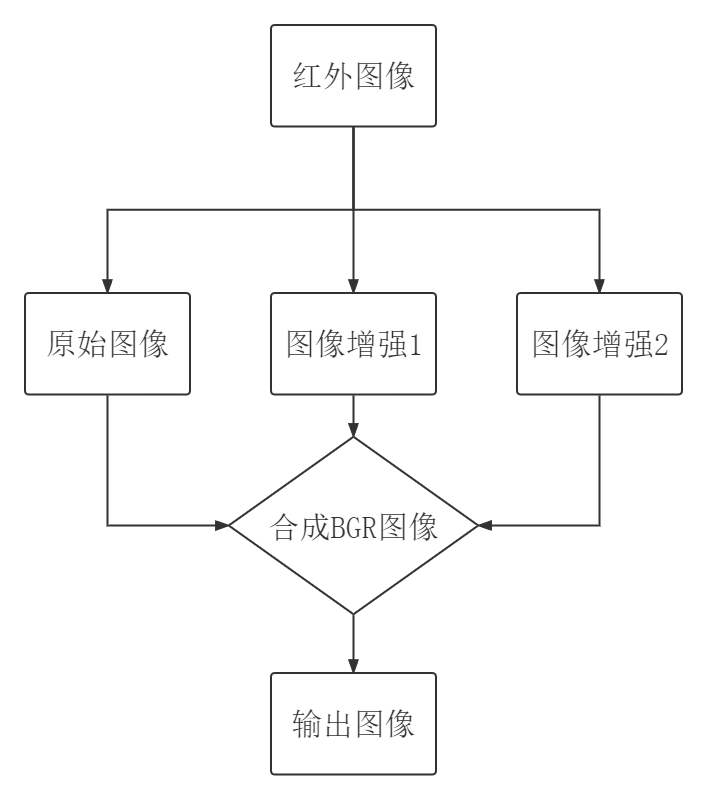
\includegraphics[width = 0.6\textwidth]{通道填充流程图.png}
  \caption{通道填充算法流程图}
  \label{tdtc}
\end{figure}

首先将输入的图像分别进行两次图像增强处理,然后将增强后的图像与原图
进行融合,融合成三通道图片,由于不能准确知道哪些增强方法会使检测结果提
高,因此采取多种增强方法进行对比实验,包括以下方法:

(1)Inversion。主要目的在于网络初始化权重为在可见光图像进行预训练
后的权重,因此将红外图像进行 Inversion 处理后,能够更接近可见光图像的灰
度图,从而达到提升检测效果的目的。

(2)CLAHE。与直方图均衡相似,只是处理的区域由原图变得更细,增强
对比度的同时,能够抑制噪声。CLAHE窗口大小选择 3*3。

(3)USM变换。主要目的在于抑制噪声的同时进行图像的锐化,强化目标的边缘。本文使用高斯模糊后的USM变换进行锐化。

\begin{figure}[htbp]
	\centering
	\begin{minipage}{0.49\linewidth}
		\centering
		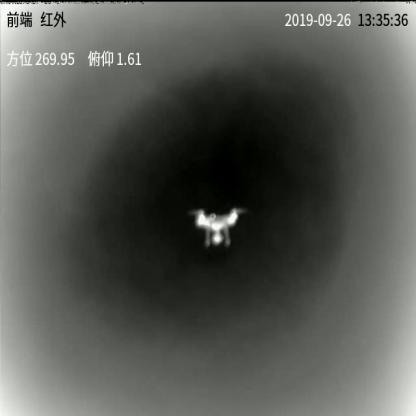
\includegraphics[width=0.9\linewidth]{原图1.JPG}
		\caption{原图示例}
		\label{txzq11}%文中引用该图片代号
	\end{minipage}
	\begin{minipage}{0.49\linewidth}
		\centering
		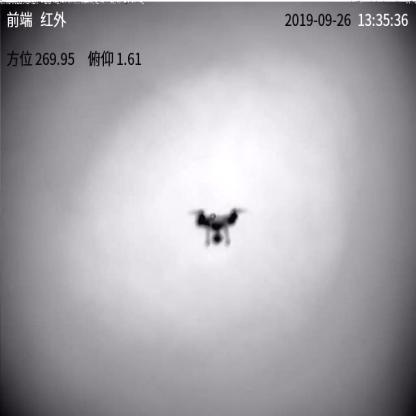
\includegraphics[width=0.9\linewidth]{inv1.JPG}
		\caption{Inversion处理示例}
		\label{txzq21}%文中引用该图片代号
	\end{minipage}
	%\qquad
	%让图片换行,
	
	\begin{minipage}{0.49\linewidth}
		\centering
		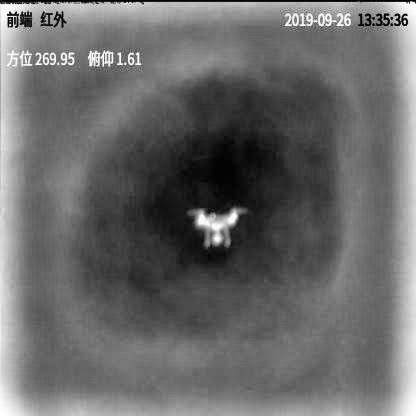
\includegraphics[width=0.9\linewidth]{clahe1.JPG}
		\caption{CLAHE处理示例}
		\label{txzq31}%文中引用该图片代号
	\end{minipage}
	\begin{minipage}{0.49\linewidth}
		\centering
		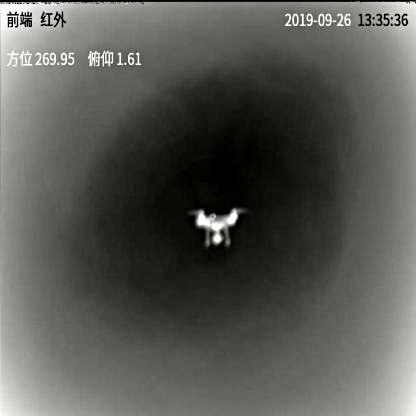
\includegraphics[width=0.9\linewidth]{usm1.JPG}
		\caption{USM处理示例}
		\label{txzq41}%文中引用该图片代号
	\end{minipage}
  \label{txzq}
\end{figure}

增强后的图片效果如图\ref{txzq}所示,其中\ref{txzq11}表示原图像,\ref{txzq21}表示原图经过Inversion处理后的图像,\ref{txzq31}表示原图像经过CLAHE处理后的图像,\ref{txzq41}表示原图像经过USM处理后的图像。

\subsection{图像拼接算法}
由于在红外无人机目标检测的场景下,小尺度目标(面积占整个图像总面积比例较小)的数量占比较大,因此考虑采用一种图像拼接的数据增强算法,将训练数据中的小目标增多,同时丰富训练数据图像中的背景,增强模型的泛化能力,从而增强网络对小目标的检测能力。

该算法的实现方法是,从训练集中随机抽取4个图像,将这4张图像进行拼接后生成一张与原始图像相同大小的新图像输入网络。

\begin{figure}[htbp]
	\centering
	\begin{minipage}{0.49\linewidth}
		\centering
		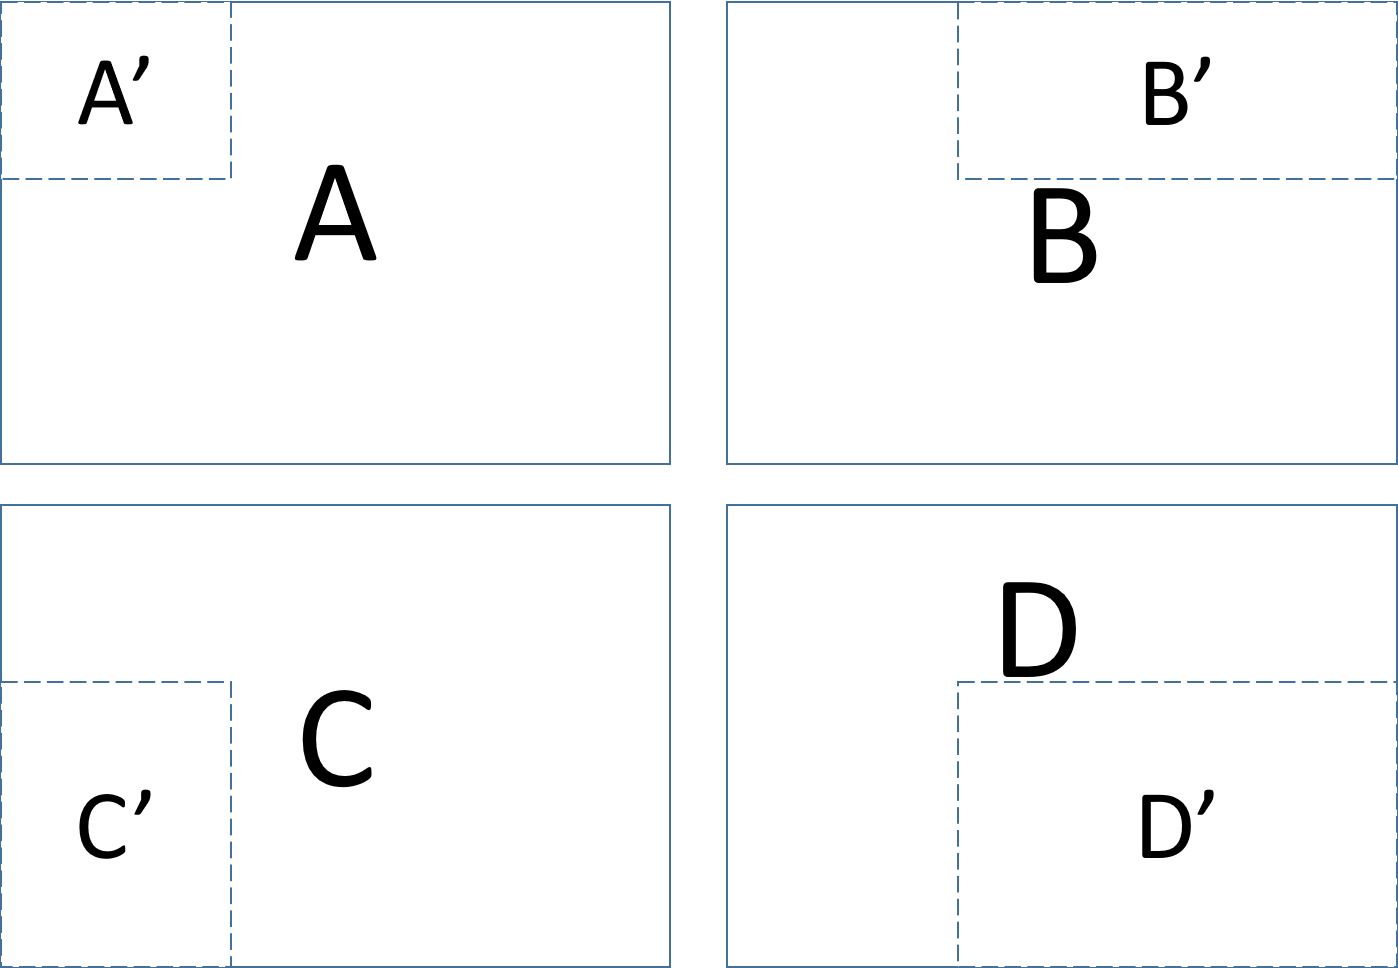
\includegraphics[width=0.9\linewidth]{txpj1.PNG}
		\caption{原始图像及切割示意图}
		\label{txpj1}%文中引用该图片代号
	\end{minipage}
	%\qquad
	\begin{minipage}{0.49\linewidth}
		\centering
		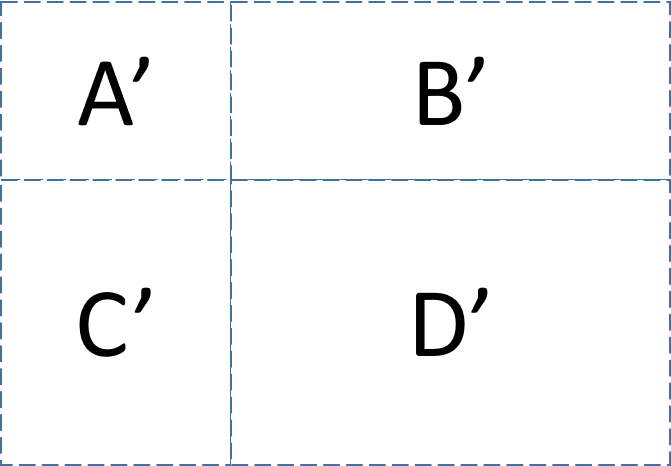
\includegraphics[width=0.9\linewidth]{txpj2.PNG}
		\caption{拼接结果图}
		\label{txpj2}%文中引用该图片代号
	\end{minipage}
\end{figure}

如图\ref{txpj1}所示,图像拼接算法的实现流程是:

(1)图中A、B、C、D分别是4张大小尺寸相同的原始图像,假设长为$w$,宽为$h$。

(2)在图像矩形的中心区域范围内随机生成一个坐标作为四张图片的切割点(例如生成点坐标为$(x,y)$,则限制其中$x\in[0.4w,0.7w],y\in[0.4h,0.7h]$)。

(3)将每张图片分割成四个矩形后,取每张图片的不同部分,即在图A中取A'(原图A的左上部分),在图B中取B'(原图B的右上部分),在图C中取C'(原图C的左下部分),在图D中取D'(原图D的右下部分)。

(4)将4张小图按其在原图中的位置放置后得到结果图,如图\ref{txpj2}所示。

如图\ref{txpj}所示,对随机4张红外无人机数据图像应用图像拼接算法后得到一张包含更丰富背景、更多标注目标、更小尺寸目标的训练样本图。

\begin{figure}[htpb]
  \centering
  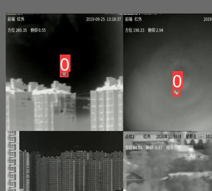
\includegraphics[width = 0.5\textwidth]{图像拼接1.png}
  \caption{图像拼接效果图}
  \label{txpj}
\end{figure}

\section{改进损失函数}
YOLOv5的损失函数由三部分组成:第一部分是bounding box损失,主要根据预测目标框和真值目标框的重合程度进行计算。第二部分是置信度损失,第三部分是分类误差。

其中对于bounding box的损失函数主要是基于$IoU$(交并比,Intersection over Union)进行计算。$IoU$一般表示预测框与真值框面积的交并比,即二者相交的面积除以二者所占的总面积。
\begin{equation}
  I o U=\frac{|A \cap B|}{|A \cup B|}
\end{equation}

这样一种计算方式相对于之前的基于点到点之间距离的MSE损失函数已经有较大的优势,主要体现在:

(1)MSE损失函数由于是按点距离计算,因此对于任务目标的尺寸变化较为敏感,尺寸变化往往会引起损失函数的无意义波动。

(2)MSE损失函数从点距离出发,忽略了目标框各点之间的关联。因此基于$IoU$的损失函数已经在一定程度上反映了预测框与真值框之间的误差关系。

而$IoU$损失函数有两个重要特性,使得它能作为很多计算机视觉算法的损失函数。

(1)$\mathcal{L}=1-IoU$满足非负性、同一性、对称性、三角不等性等所有损失函数的特性。

(2)$IoU$相对于问题的规模是不变的。这意味着两个任意形状之间的相似性独立于它们的空间规模。

然而基于$IoU$的损失函数也存在一定的问题。

(1)当预测框与真值框没有相交区域时,$IoU$值为0,此时损失loss为0,无法进行梯度回传,也就是无法进行模型训练。

(2)$IoU$还是无法精确地衡量预测框与真值框之间的误差情况,尤其是在$IoU$为0时,预测框与真实框之间的距离变得无法量化。

因此,针对$IoU$的这一问题,为了增强算法对红外无人机目标检测任务中的目标框定位能力,可以引入一种更加完善的$GIoU$损失函数。设$I o U=\frac{\mathcal{I}}{\mathcal{U}}$
,其中$\mathcal{I}$表示预测框与真值框相交部分面积,$\mathcal{U}$表示预测框与真值框合并部分面积,则$GIoU$的计算公式是:
\begin{equation}
  G I o U=I o U-\frac{A^{c}-\mathcal{U}}{A^{c}}
\end{equation}

其中$A^{c}$表示预测框和真值框的最小闭包区域的面积。

\begin{figure}[htbp]
  \centering
  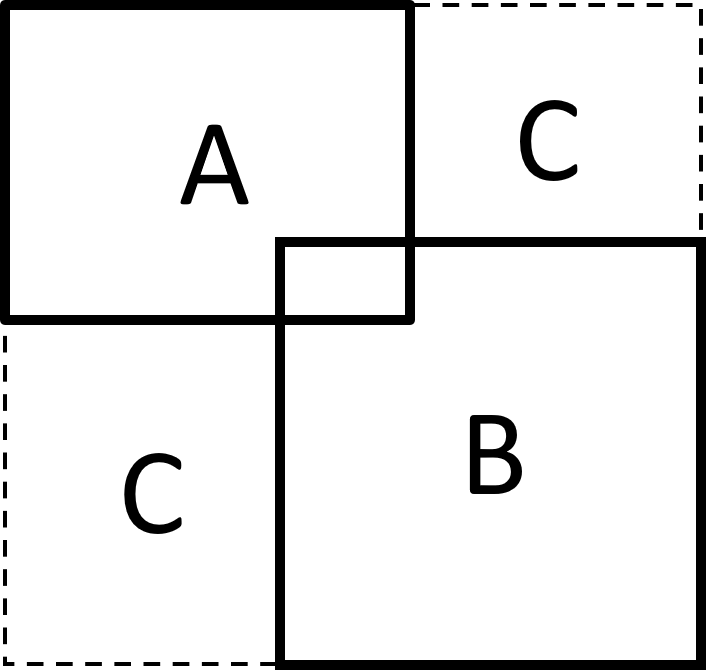
\includegraphics[width = 0.5\textwidth]{giou示意.png}
  \caption{GIoU示意图}
  \label{gi}
\end{figure}

如图\ref{gi}所示,$GIoU$的计算流程是:

(1)找到预测框(图\ref{gi}中区域A)和真值框(图\ref{gi}中区域B)的边界点,计算闭包区域(图\ref{gi}中整个虚线包围的矩形区域)面积。

(2)计算预测框和真值框相交部分和合并部分面积,求得补集部分(图\ref{gi}中区域C)面积。

(3)代入公式$G I o U=I o U-\frac{A^{c}-\mathcal{U}}{A^{c}}$以及$\mathcal{L}_{G I o U}=1-G I o U$得到$\mathcal{L}_{G I o U}$。

$GIoU$是经过改进的$IoU$计算方法,有如下几个特点:

(1)与$IoU$相似,也是一种距离度量,作为损失函数满足损失函数的需求。

(2)$GIoU$除了关注重叠区域不同,还关注了非重叠区域,能够更好的反应重合度。

(3)$GIoU$对目标的尺度不敏感。

(4)当预测框与真值框重合时,$GIoU=IoU$,即$GIoU$的上限是$IoU$,因此训练时不会出现梯度爆炸的情况。

\section{实验结果与分析}
本节将在YOLOv5网络的基础上,应用本章提出的数据增强算法以及损失函数的改进方案,在自建红外无人机目标数据集上进行对比实验,并对实验结果进行分析。


\subsection{实验环境与参数}
本章提到的YOLOv5基础算法用深度学习网络框架Pytorch进行实现、训练和测试。操作系统为Windows 10,使用的主要软件为python。实验平台采用的CPU型号为Intel Core i7-11700k,GPU型号为NVIDIA GeForce RTX 3080Ti,显存容量为12GB。训练过程中使用GPU进行加速。

\subsection{不同算法对比与分析}
在上述环境下,进行算法的训练和测试,以mAP和推理时间作为评价指标,对比结果列在表\ref{m1}中。

\begin{table}[htbp]
  \caption{不同算法对红外无人机数据集的检测结果}
  \vspace{0.5em}\centering\wuhao
  \begin{tabular}{ccc}
  \toprule
  检测算法 & mAP\\
  \midrule
  YOLOv5 & 269.8\\
  Ours(YOLOv5+Inversion数据增强) & 421.0\\
  Ours(YOLOv5+CLAHE数据增强) & 640.2\\
  Ours(YOLOv5+USM数据增强) & 640.2\\
  Ours(YOLOv5+Inversion+CLAHE通道填充) & 640.2\\
  Ours(YOLOv5+Inversion+USM通道填充) & 640.2\\
  Ours(YOLOv5+CLAHE+USM通道填充) & 640.2\\
  Ours(YOLOv5+Inversion+CLAHE通道填充+图像拼接) & 640.2\\
  Ours(YOLOv5+Inversion+CLAHE通道填充+GIoU) & 640.2\\
  Ours(YOLOv5+Inversion+CLAHE通道填充+图像拼接+GIoU) & 640.2\\
  \bottomrule
  \end{tabular}
  \label{m1}
\end{table}

由表\ref{m1}中所示数据可以看出,YOLOv5目标检测算法在本文的检测任务中已经能取得较好的精度。本节首先对基础的数据增强方法进行了对比实验(即对训练数据采用Inversion变换、CLAHE变换、USM变换其中之一处理后生成训练数据)。实验结果显示,在进行Inversion数据增强后,YOLOv5算法的检测精度得到了小幅度的提升,这是由于部分图像在经过Inversion后和原始图像相差较大,使得网络学习到了更为丰富的特征。而应用CLAHE数据增强方法后算法的检测精度基本不变,应用USM数据增强方法后算法的检测精度略有下降,这是因为USM虽然在一定程度上抑制噪声,但是由于有些图像本身的信噪比不高,有相当数量的图像经过USM后增强了噪声,影响了模型的训练效果。随后本节对本文提出的通道填充算法进行了对比实验。实验结果显示,YOLOv5+Inversion+CLAHE通道填充取得了相比于单纯应用Inversion数据增强后的YOLOv5网络取得了更高的检测精度,这是因为网络在经过不同的三通道数据进行训练后增强了特征提取的能力。在应用了图像拼接算法后,算法的精度并没有提高,虽然理论上模型对小目标的检测能力得到增强,但是本文采用的训练集已经包含了大量的小目标样本,因此单纯应用图像拼接后可能一定程度上降低了模型的泛化能力。而后本节对应用了GIoU损失函数的网络结构进行了对比实验,结果显示YOLOv5+Inversion+CLAHE通道填充+图像拼接+GIoU的红外无人机目标检测算法取得了比其他算法更高的检测精度,这一方面是因为GIoU损失函数的改进提高了网络对于目标预测框的定位能力,另一方面是因为图像拼接后,目标框和预测框更容易出现更大的偏差,原始的IoU损失函数性能下降,因此图像拼接算法在配合GIoU损失函数后表现出了更高的检测精度。

\section{本章小结}
本章首先介绍了本文采用的自建红外无人机目标数据集的制作过程。之后本章介绍了本文采用的目标检测算法基于的YOLOv5神经网络的结构,并且在数据集上进行了对比实验,证明了在红外无人机目标检测任务中,YOLOv5算法的检测能力强于常见的YOLOv3算法、Faster-RCNN算法以及SSD算法。此后本章分析了本课题主要面临的问题,其一是本课题的目标检测应用场景是红外图像,其二是无人机目标检测场景下待测目标常常以小目标形式出现。针对这两个问题本章提出了一种数据增强算法,即在训练过程中通过特定的图像处理方法增强模型的训练效果,并且进行了对比试验,验证了对模型的改进效果。此外本章对YOLOv5采用的bbox损失函数进行了改进,进一步增强了本文提出算法在红外无人机数据集上的检测精度。









% Local Variables:
% TeX-master: "../main"
% TeX-engine: xetex
% End:
